\subsection{Exact geometric occupation and the directional lower}
\label{sec:geometry-12}

The atomic square extends to the actual constant-lapse metric, with its
kinetic form $K_\nu=\tau\nu\|\nabla_g\cdot\|^2$ and measure
$\nu^{-1}r^2\dd r\dd\Omega$, $0<\nu\le1$. The complete scalar Coulomb
spectrum has negative levels
\begin{equation}
 -\frac{C^2}{4\tau\nu^3(n_r+\alpha_l+1)^2},\qquad
 \alpha_l(\alpha_l+1)=l(l+1)/\nu^2,
\end{equation}
with spin-angular multiplicity $2(2l+1)$. Let $w_{n,\nu}$ sum the $n$
largest inverse squared denominators. Matching every $(n_r,l)$ label to
its flat counterpart gives $w_{n,\nu}\le w_n$. For $n\le6$, omitted
$l\ge3$ or $n_r\ge3$ have denominators at least four, while six included
s-wave slots have denominators at most three. This establishes complete
occupation without an angular-cutoff assumption.\samref{REF12_TWO}

\begin{table}[htbp]\centering\small
\caption{Complete geometric occupation through six electrons.
At $\nu=3/4$, write $s=\sqrt{137}$.}
\begin{tabular}{crrr}\toprule
$n$&$w_{n,1}$&$w_{n,3/4}$&$w_{n,1/2}$\\\midrule
1&1&1&1\\2&2&2&2\\3&$9/4$&$9/4$&$9/4$\\
4&$5/2$&$5/2$&$5/2$\\
5&$11/4$&$(5777-27s)/2048$&$47/18$\\
6&3&$(3217-27s)/1024$&$49/18$\\\bottomrule
\end{tabular}\label{tab:geometry-weights-12}
\end{table}

The matched directional profile uses
$d=2(\nu+1)/\nu$, $h=dr/[(d+1)r_c]$ inside the core and
$h=1-(r_c/r)^d/(d+1)$ outside. Splitting the same kinetic form between
the scalar occupation and directional square yields
\begin{equation}
 E_{e,n}\ge-
 \frac{[C\sqrt{w_{n,\nu}}+A\nu\sqrt n/(\nu+1)]^2}
      {4\tau\nu^3}.
\label{eq:geometry-directional-12}
\end{equation}
The optimization uses
$a^2/\theta+b^2/(1-\theta)-(a+b)^2
=[a-(a+b)\theta]^2/[\theta(1-\theta)]$.
Take its pointwise maximum with the original geometric spectral branch
$-w_{n,\nu}(C+A)^2/(4\tau\nu^3)$ and core floor $-n(C+A)/r_c$,
then minimize the complete nuclear source. The earlier flat-weight
directional comparison remains valid, but its universal strict-improvement
claim against the geometric weight was false. The new exact-weight branch
repairs that comparison and is stronger than the geometric spectral
branch for $A>0$, $n\le6$. A dominating core floor can erase the gain.

This last possibility is realized throughout the nonflat published panel.
At $\nu=3/4,1/2$, $C\in\{2,6\}$ and $1\le n\le C$, the ratio of the
directional spectral cost to the positive core-floor cost has a strictly
positive minimum excess for every $A\ge0$. Thus the maximum is exactly
the core floor for all 88 nonflat populated accounts. At $\nu=1$ the
weights already agree. The exact-weight refinement changes zero of 132
final lower accounts relative to the valid three-way maximum. Against
the original geometric/core comparison there are 17 improved flat accounts.
These are exact dominance conclusions, not numerical equality tests.

The all-132 reconstruction retains all ten helium and 51 carbon $q/I$
classes. The available explicit spherical-shell portfolio has 30 positive
ionization lower endpoints and 102 overlaps. Its shell additions obey
\begin{equation}
 \Delta U_j\le10\nu^3/R^2-(Z-j+1)J_1/R
              +\frac{g_pM_{\alpha_1}}{(2\alpha_1+1)R^{\alpha_1+1}},
\end{equation}
where $J_1=30(4\log2-11/4)$ and
$M_\alpha=\sum_{i<j}(2R_i)^\alpha$. Radii begin at two and double to a
negative increment, then quadruple for the next shell. The interval
$[L_{n-1}-U_n,U_{n-1}-L_n]$ uses matching source minima throughout.
All 132 endpoint boxes are retained in the report and machine-readable
evidence; they are not substituted for the missing historical flat CI
portfolio.

The two absent historical endpoint files have known hashes but unavailable
operands in this window. The upgraded retained-CI count is consequently
only bounded between 30 and 40. The ten unresolved possible additions are
He4 covers3/4 at $n=2$, both couplings, and carbon333/343/444 at $n=5,6$,
weak polarization. Restoring those endpoints suffices to settle that count.
Neither the exact lower table nor the complete spherical count is missing.
A reachable $l=1$, $\nu=1/2$ control rejects the false flat centrifugal value: its coefficient residual is six. Constant $\nu$ and quadratic kinetic are essential; variable lapse requires
the additional weighted-divergence derivatives, and the bound does not
automatically transfer to the smaller massive square-root kinetic.

\subsection{A rigid rotor removes the first-order orientation mean}
\label{sec:rotor-12}

The existing clamped-source $D^{-1}$ attraction and moving-reference
construction retain their earlier hypotheses. A separately specified
rotational extension fixes neutral rigid atomic preparations and adds
$H_0=B_A L_A^2+B_B L_B^2$, $B_A,B_B>0$, on normalized
$L^2(SO(3)\times SO(3))$. For the product singlet $\Omega=1\otimes1$,
the first coefficient is
\begin{equation}
 C_1=\tfrac1{10}\{(R_Av_A)\cdot(R_Bv_B)
                   +e\cdot(R_At_A-R_Bt_B)\}.
\end{equation}
Haar invariance gives $\langle C_1\rangle=0$. Its three images of
$\Omega$ lie in orthogonal angular sectors $(1,1),(1,0),(0,1)$, with
squared norms $|v_A|^2|v_B|^2/300$, $|t_A|^2/300$, $|t_B|^2/300$ and
gaps $2(B_A+B_B),2B_A,2B_B$. The full second-order response is therefore
\begin{equation}
 -\frac{S_2}{D^2},\quad
 S_2=\frac1{600}\left\{
 \frac{|v_A|^2|v_B|^2}{B_A+B_B}
 +\frac{|t_A|^2}{B_A}+\frac{|t_B|^2}{B_B}\right\}.
\label{eq:rotor-second-12}
\end{equation}
The complete singlet image is included, so this coefficient needs no
angular truncation. Bounded $C_1$ and the rotor gap justify perturbation
at sufficiently large $D$ for each fixed positive $B_A,B_B$.
\samref{REF12_TWO}

For any correlated normalized $n$-electron preparation,
$|\sum_i\langle n_i\rangle|\le n$, whence $|v|\ge|U|-n$.
Thus neutral carbon 444 has $|v_C|\ge6$ and the stated oxygen source
$|v_O|\ge8$, independently of orbital approximation. At equal $B=1$,
their monopole contributions are at most $-27/(25D^2)$ and
$-256/(75D^2)$. A raw 15-coordinate Haar-Gram resolvent independently
checks the exact sector gaps. Replacing the pair gap four by the
single-rotor gap two doubles the carbon term and is a rejected control.
Without neutral charge allocation a scalar $D^{-1}$ term remains.

\subsection{The complete inverse-square coefficient retains the Taylor term}
\label{sec:rotor-full-tail-12}

Vanishing first mean does not make the whole molecular coefficient equal
to $-S_2$. For the original common direction, put $c=n\cdot e$ and expand
\begin{equation}
\begin{split}
 n_D={}&n+D^{-1}r(cn-e)\\
      &+D^{-2}r^2\{(7c^2-1)n/2-3ce\}+O(D^{-3}).
\end{split}
\end{equation}
Haar averaging the full original second Taylor term gives
\begin{equation}
\begin{split}
 K_2=\frac13\sum_{a=A,B}\bigg\{&g_p\sum_{i\in a}
   \left\langle\frac{r_i^2\,U_a\cdot n_i}{\max(r_i,r_c)}\right\rangle\\
 &+v_p\sum_{i<j\in a}\left\langle
 \frac{r_ir_j(1+c_{ij}^2)-(r_i^2+r_j^2)c_{ij}}
 {|x_i-x_j|}\right\rangle\bigg\}.
\end{split}
\end{equation}
Correlated pair expectations include exchange. Electron polarization self
is constant because the exact direction has unit norm; scalar own-core
terms are independent of $D$. The original cross-center second means
vanish by the independent Haar averages, rather than being omitted.
For compact rigid preparations the Taylor expansion and averaged remainder are uniform at sufficiently large $D$. The retained normalized localization extends this to exponentially decaying states with the required finite radial moments. The complete clamped rigid expansion is
\begin{equation}
 E(D)-E(\infty)=(K_2-S_2)D^{-2}+o(D^{-2}).
\end{equation}
Reachable pair numerators $714/625$ and $-1$, and an own-core witness
$12/25$, exclude a universal sign shortcut for $K_2$.

There is nevertheless a useful full-tail sufficient bound. With
$u=(r-s)^2$, $v=2rs(1-c)$ and $d^2=u+v$, the pair numerator is
$N_2=-cu+(1-c)v/2$, so $|N_2|\le d^2$.
Consequently, for $\mathcal R_a=\sum_i\langle r_i\rangle$,
\begin{equation}
 |K_2|\le\tfrac13\sum_{a=A,B}
              [g_p|U_a|+v_p(n_a-1)]\mathcal R_a.
\end{equation}
At weak polarization and equal per-atom radial sums
$\mathcal R_A=\mathcal R_B=R$, a negative complete coefficient follows
for identical carbon 444 if $0<B<81/(85R)$, and for the stated oxygen
source if $0<B<256/(115R)$. These conditions retain the Taylor remainder
comparison. They do not require $t_A,t_B$ to vanish, and take large $D$
after fixing $B$, not a uniform joint $B\to0$, $D\to\infty$ limit.

For independent classical Haar orientations, the free-energy coefficient
instead is
\begin{equation}
 K_2-\frac\beta{600}
       (|v_A|^2|v_B|^2+|t_A|^2+|t_B|^2).
\end{equation}
The corrected finite thermal witness is $-1321/600$ for its $C_1$ part;
the earlier $-673/300$ used a superseded variance operand. Rotor constants,
temperature, rigid realization, internal excitations, moving dissociation
reference and recoil/rotation apparatus are separate model inputs. These
conditional $D^{-2}$ tails are not a derived $D^{-6}$ molecular law or a
physical-unit calibration.

\begin{figure}[htbp]\centering
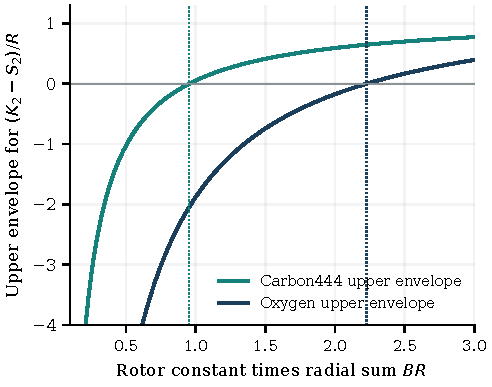
\includegraphics[width=\columnwidth]{refinement_20261112/figures/rotor_tail.pdf}
\caption{A sufficient full-tail comparison for identical rigid atoms at
weak polarization. The displayed upper envelopes bound $(K_2-S_2)/R$;
a negative envelope guarantees attraction in that specified rotor model.
Horizontal coordinate is $BR$, with $R$ the per-atom sum of electron
radii. No measured molecular parameters enter.}
\label{fig:rotor-tail-12}
\end{figure}
